\section{CAPE Framework}
\label{equity-sec:cape}

\gls{CA} is one of the possible frameworks to address the balance problem of diverse sources of inequalities. But there is one of these frameworks that arises inside \gls{CEd} area and tries to address this same complex problem: \gls{CAPE} framework \cite{fletcher:2021}. It provides a set of essential constructs to conduct \gls{CEd} equity analysis to supply stakeholders with more qualified information to help their decision-making.

It stands for four expressions: \acrfull{CAPE}. It proposes to assess \gls{CEd} using strategic questions at more diverse levels of analysis (Figure \ref{fig:cape-framework}). The \gls{CAPE} richness is that each one of these expressions represents an education level which \gls{CEd} can be offered, allowing to tackle equity issues as a public policy perspective transversally.

\begin{figure}[ht!]
\centering

\caption{\textmd{The \acrshort{CAPE} Framework schema.}}
\label{fig:cape-framework}
\fcolorbox{gray}{white}{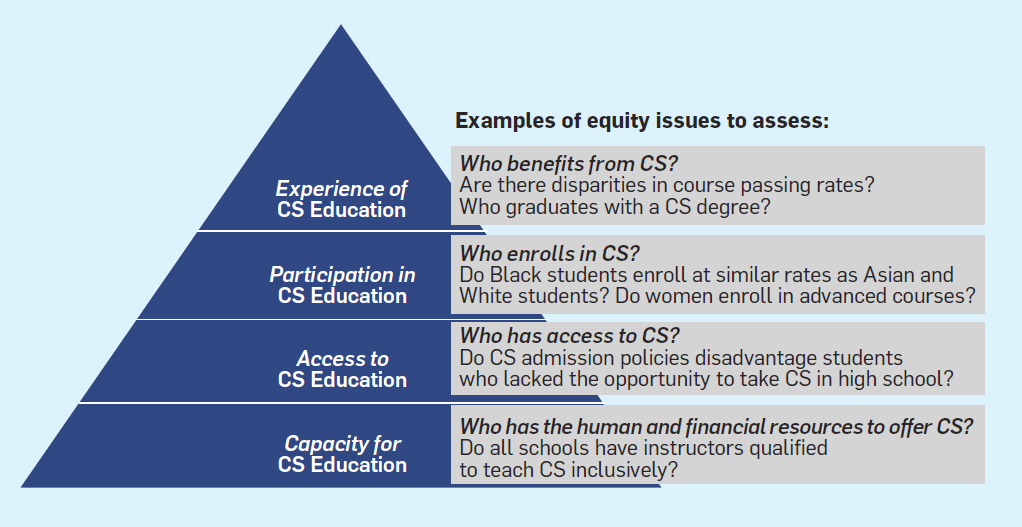
\includegraphics[width=0.9\textwidth]{images/chapter-03/cape-framework.png}}

\par\medskip\ABNTEXfontereduzida\selectfont\textbf{Source:} \citeonline{fletcher:2021}.
\end{figure}

"C" represents the capacity for offering \gls{CS} education that schools have. In this framework, it is materialized from indicators that signal to the human, material, and infrastructure dimensions. Typical questions of capacity are: "Which types of schools have teachers with the requisite skills to teach \gls{CS} courses? (ii) Do schools in low-income communities have sufficient resources to start \gls{CS} programs? (iii) Are there location-based disparities in terms of which districts are able to recruit and train \gls{CS} teachers?" \cite[p.~4]{warner:2022}.

"A" represents the access to \gls{CS} education that schools provide. While "C" represents structure, "A" represents the next step of the process: access. Both "C" and "A" refer to the basic education level. Indicators such as the number of members of disadvantaged communities who have access (or not) to \gls{CS} education. Typical questions of access are: "(i) Do \gls{CS} admission policies disadvantage students who lacked the opportunity to take \gls{CS} in high school?" (Figure \ref{fig:cape-framework}), "(ii) What is the relationship between the number of \gls{CS} courses that schools offer and the proportion of students who are economically disadvantaged?" \cite[p.~10]{warner:2022}.

"P" represents the participation in \gls{CS} education concerning the proportions of students who enrolled in \gls{CS} courses for different subgroups. Indicators such as the number of members of disadvantaged communities who participate in (or no) \gls{CS} courses. Typical questions of participation are: "(i) Do Black students enroll at similar rates as Asian and White students? (ii) Do women enroll in advanced courses?" (Figure \ref{fig:cape-framework}). 

Lastly, "E" represents the experience of \gls{CSE} students. While "P" represents participation (similar to access), "E" represents \gls{CSE} students' experience (including data related to number of graduates). Both "P" and "E" refer to the higher education level. Indicators about how "to quantitatively assess and monitor issues of equity regarding students’ learning experiences in \gls{CS}" \cite[p.~5]{warner:2022}. Typical questions of experience are: "(i) Are there disparities in course passing rates? (ii) Who graduates with a \gls{CS} degree?" (Figure \ref{fig:cape-framework}).

Although \gls{CAPE} can map important variables to an equity analysis, the concept
of 'capacity' is strongly related to resources, ignoring some essential aspects relative to the real opportunities for a computing student. Furthermore, in developing countries, other challenges emerge. Beyond the potential inequity sources that emerged from natural diversity in the classroom (e.g., gender, race), structural barriers deepen the situation (e.g., socioeconomic status, poverty). In African countries, for instance, it used the \gls{CAPE} framework to analyze equity issues in \gls{CEd} \cite{tshukudu:2023}. Although the authors highlight the strengths of its use, they also point out some limitations: 
\begin{citacao}
    ``The \gls{CAPE} framework helps map the progression from 'Capacity for' to 'Experience of' computer science education as a route to equity, but in order to support development in low and middle income countries, it may be helpful to have the capacity level finely grained'' \cite[p.~1]{tshukudu:2023}.
\end{citacao}
Maybe the \gls{CA} can help to fill some gaps during equity analysis using only the \gls{CAPE} framework. 